\begin{frame}{\subsecname: Schema del sistema}
    \begin{figure}
        \centering
        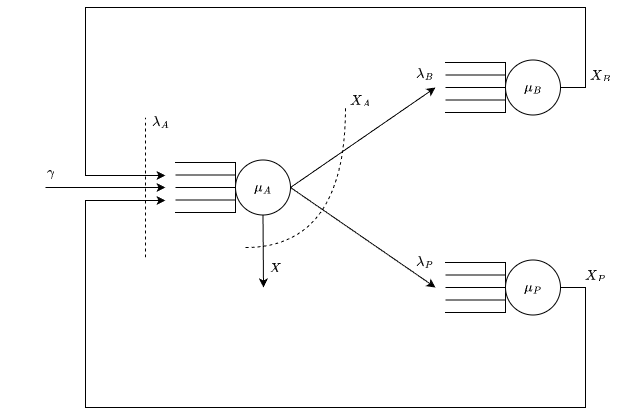
\includegraphics[width=0.75\linewidth]{figs/webapp_conceptual.drawio.png}
        \caption{Diagramma a reti di code del sistema.}
        \label{fig:enter-label}
    \end{figure}
\end{frame}

\begin{frame}{\subsecname: Job e classi}
    Ai job è stata assegnata una classe seguendo il seguente criterio:
    \begin{itemize}
        \item \textbf{Classe 1}: job in arrivo dall'esterno, restano in questa classe fino all'ingresso in servizio in $B$.
        \item \textbf{Classe 2}: job in arrivo al server $A$ tramite feedback del server $B$, restano in questa classe fino all'ingresso in servizio in $P$.
        \item \textbf{Classe 3}: job in arrivo al server $A$ tramite feedback del server $P$. Questa classe include i job che escono dal sistema.
    \end{itemize}
\end{frame}

\begin{frame}{\subsecname: Variabili di stato}
    Le variabili di stato che meglio descrivono il sistema sono:
    \begin{itemize}
        \item $N_{\text{node, class}}$: numero di job di classe \textit{class} $\in \{1,2,3\}$ nel nodo \textit{node} $\in \{A,B,P\}$.
        \item $C_j \, \text{con } j \in [0, \infty)$: valore che indica la classe di appartenenza del job $j$.
    \end{itemize}
    La simulazione utilizzata è una \textit{next-event simulation}. Gli eventi sono:
    \begin{itemize}
        \item \textbf{Arrival}: caratterizzati da server di destinazione e classe del job in arrivo.
        \item \textbf{Departure}: caratterizzati da server di partenza e classe del job in partenza.
    \end{itemize}
\end{frame}

\begin{frame}{\subsecname: Evoluzione degli eventi}
    Gli eventi nei server \( A \), \( B \), e \( P \) seguono un pattern generale:
    \begin{itemize}
        \item \textbf{Arrival:}
        \begin{itemize}
            \item Incremento della variabile di stato del nodo relativo, \( N_{\text{node,class}} \).
            \item Generazione dell'evento \textit{Departure} per il job appena arrivato.
            \item Se l'arrivo è dall'esterno $C_j$ viene posta ad 1.
        \end{itemize}
        \item \textbf{Departure:}
        \begin{itemize}
            \item Decremento della variabile di stato \( N_{\text{node,class}} \).
            \item Incremento della variabile $C_j$.
            \item Generazione di un evento \textit{Arrival} nel nodo successivo o uscita dal sistema (se il job è di classe 3 in \( A \)).
        \end{itemize}
    \end{itemize}
\end{frame}